\documentclass[11pt]{article}

\usepackage[a4paper,margin=1in]{geometry}
\usepackage{amsmath}
\usepackage{booktabs}
\usepackage{graphicx}
\usepackage{hyperref}
\usepackage{enumitem}
\usepackage{array}
\usepackage[T1]{fontenc}

\setlength{\parindent}{0pt}
\setlength{\parskip}{0.55em}
\setlist[itemize]{leftmargin=1.4em,itemsep=0.15em,topsep=0.2em}
\newcolumntype{L}[1]{>{\raggedright\arraybackslash}p{#1}}
\graphicspath{{../plots/nu-scattering/}{plots/nu-scattering/}{figures/}{docs/figures/}}

\title{CSpack Kernel and Scattering-Matrix Library}
\author{}
\date{September 2026}

\begin{document}
\maketitle

\section{Purpose}

CSpack evaluates energy redistribution kernels for photon-electron Compton
scattering and neutrino scattering on electrons and positrons in isotropic
media. The library provides fixed-scatterer kernels, thermal averages over
electron or positron distributions, kernel moments, compressed spline
representations, and scattering matrices for repeated-scattering solvers.

The photon part follows Sarkar, Chluba and Lee (2019), the CSpack Compton
kernel paper \cite{SarkarChlubaLee2019}. The neutrino extension follows
Chluba, Cyr, Uwabo-Niibo and Yamaguchi (2026), where the isotropic
neutrino-electron kernel is reduced from the full collision integral to a
compact kernel form and added to CSpack \cite{ChlubaCyrUwaboNiiboYamaguchi2026}.

CSpack is a library rather than a standalone evolution solver. The example
program \texttt{CSpack\_main.cpp} illustrates common calls, while
\texttt{CSpack/CSpack.h} collects the public C++ headers. A small C interface is
declared in \texttt{CSpack/CSpack\_c.h} for integration weights and photon
scattering matrix setup.

\section{Variables and Normalization}

The main routines use dimensionless variables:
\begin{center}
\small
\begin{tabular}{L{0.17\linewidth}L{0.22\linewidth}L{0.50\linewidth}}
\toprule
Symbol & Code name & Meaning \\
\midrule
$\omega_0$, $\omega_1$ & \texttt{omega0}, \texttt{omega1} & Incoming photon or neutrino energy in units of $m_ec^2$. \\
$\omega$, $\omega_3$ & \texttt{omega}, \texttt{omega3} & Outgoing photon or neutrino energy in units of $m_ec^2$. \\
$p_0$, $p_2$ & \texttt{p0}, \texttt{p2} & Scatterer momentum in units of $m_ec$. \\
$\gamma$ & \texttt{gamma\_f(p)} & Electron or positron Lorentz factor $\sqrt{1+p^2}$. \\
$\Theta$ & \texttt{theta}, \texttt{The} & Scatterer temperature $kT_e/(m_ec^2)$. \\
$x$ & \texttt{xarr[i]} & Grid energy, usually $\omega/\Theta_g$. \\
$\mu_e$ & \texttt{mue} & Electron chemical potential parameter used by the FD routines. \\
\bottomrule
\end{tabular}
\end{center}

The low-level photon kernels return the redistribution shape with the Thomson
normalization factored out. The low-level neutrino kernels return the
redistribution shape after factoring out the reference weak-scattering
normalization used in the neutrino-kernel paper. The neutrino matrix wrapper
adds the low-energy $x_0^2$ scaling and the optional process normalization
through \texttt{sigma\_norm}.

\section{Building}

The repository builds through the top-level \texttt{Makefile}, which delegates
to \texttt{Makefile.in}.
\begin{verbatim}
make lib
make bin
\end{verbatim}
\texttt{make lib} creates \texttt{libCSpack.a}. \texttt{make bin} also links
the example program \texttt{CSpack\_main}. The default \texttt{Makefile.in}
expects GSL and Boost headers/libraries under the configured Homebrew paths and
enables OpenMP through \texttt{g++}.

For external C++ code, include the umbrella header and link against the static
library plus the same numerical dependencies:
\begin{verbatim}
#include "CSpack.h"
\end{verbatim}

\section{Low-Level Kernel Routines}

The fixed-scatterer kernels all use the function-pointer type
\begin{verbatim}
typedef double (*kernel_ptr)(double, double, double);
\end{verbatim}
The arguments are \texttt{(incoming\_energy, scatterer\_momentum,
outgoing\_energy)}. This common signature lets photon and neutrino kernels be
passed through the same moment, FD-average, output, and representation
machinery.

\subsection{Kinematic Helpers}

\texttt{CSpack\_functions} contains the shared kinematic layer used by both
photon and neutrino kernels:
\begin{center}
\small
\begin{tabular}{L{0.40\linewidth}L{0.48\linewidth}}
\toprule
Function & Role \\
\midrule
\texttt{gamma\_f(p)}, \texttt{pfunc(gamma)} & Convert between momentum and Lorentz factor. \\
\texttt{gamma\_sc(omega0, p0, omega)} & Final scatterer Lorentz factor after an energy transfer. \\
\texttt{pfunc\_sc(omega0, p0, omega)} & Final scatterer momentum after an energy transfer. \\
\texttt{omegamin}, \texttt{omegacrit}, \texttt{omegamax} & Allowed outgoing-energy limits for fixed incoming energy and scatterer momentum. \\
\texttt{Get\_zone(omega0, p0, omega)} & Branch selector for the analytic kernel expressions. \\
\texttt{lambda\_p}, \texttt{lambda\_m}, \texttt{kappa} & Invariants and auxiliary variables used inside the kernel expressions. \\
\texttt{mb\_dist\_func}, \texttt{mb\_dist\_norm}, \texttt{pbar} & Relativistic Maxwell-Boltzmann distribution helpers for thermal averaging. \\
\bottomrule
\end{tabular}
\end{center}

These are useful for diagnostics and for checking support limits before
evaluating a kernel. Most users call the higher-level kernel functions directly.

\subsection{Photon Kernels}

\texttt{CSpack\_kernels} implements photon-electron redistribution kernels:
\begin{center}
\small
\begin{tabular}{L{0.36\linewidth}L{0.52\linewidth}}
\toprule
Function & Use \\
\midrule
\texttt{kernel\_exact(omega0, p0, omega)} & Exact isotropic Compton kernel for a fixed electron momentum. \\
\texttt{kernel\_recoil} & Recoil-dominated limiting kernel. \\
\texttt{kernel\_doppler} & Doppler-dominated limiting kernel. \\
\texttt{kernel\_ur} & Ultra-relativistic limiting kernel. \\
\texttt{kernel\_all(..., type)} & String-dispatched fixed-momentum photon kernel. \\
\texttt{Get\_kernel\_pointer(type, calling\_func)} & Returns a \texttt{kernel\_ptr} for \texttt{exact}, \texttt{recoil}, \texttt{doppler}, or \texttt{ur}. \\
\bottomrule
\end{tabular}
\end{center}

The exact kernel first checks the allowed outgoing-energy interval, chooses the
appropriate scattering zone, computes the branch variables, and evaluates the
analytic expression. Outside the allowed kinematic region it returns zero.

\subsection{Neutrino Kernels}

\texttt{CSpack\_kernels\_nu} implements neutrino scattering kernels with the
same \texttt{kernel\_ptr} signature:
\begin{center}
\small
\begin{tabular}{L{0.39\linewidth}L{0.49\linewidth}}
\toprule
Function & Process \\
\midrule
\texttt{kernel\_exact\_nue\_e} & Electron-neutrino scattering on electrons. \\
\texttt{kernel\_exact\_nue\_p} & Electron-neutrino scattering on positrons. \\
\texttt{kernel\_exact\_nue\_ep} & Sum of electron and positron targets. \\
\texttt{kernel\_exact\_numu\_e}, \texttt{kernel\_exact\_numu\_p} & Muon-neutrino scattering on electrons or positrons. \\
\texttt{kernel\_exact\_nutau\_e}, \texttt{kernel\_exact\_nutau\_p} & Tau-neutrino scattering on electrons or positrons. \\
\texttt{Get\_neutrino\_kernel\_pointer(type, calling\_func)} & Returns the process-specific \texttt{kernel\_ptr}. \\
\texttt{Get\_neutrino\_kernel\_norm(type, calling\_func)} & Coupling normalization relative to \texttt{nue\_e}. \\
\bottomrule
\end{tabular}
\end{center}

Internally, the neutrino routines evaluate the zone-dependent analytic
integrals \texttt{I20}, \texttt{I\_alpha}, and \texttt{I\_beta} with
chiral-coupling combinations \texttt{alpha\_LR} and \texttt{beta\_LR}. The
electron/positron and flavor variants are built by changing the weak couplings
rather than duplicating the kinematic machinery.

\section{Thermal Kernel Routines}

There are two thermal-averaging layers. The photon Maxwell-Boltzmann wrappers
live in \texttt{CSpack\_kernels}:
\begin{center}
\small
\begin{tabular}{L{0.40\linewidth}L{0.48\linewidth}}
\toprule
Function & Use \\
\midrule
\texttt{thermal\_kernel\_exact(omega0, omega, theta)} & Thermal average of the exact photon kernel. \\
\texttt{thermal\_kernel\_recoil}, \texttt{thermal\_kernel\_doppler}, \texttt{thermal\_kernel\_ur} & Thermal averages of the limiting photon kernels. \\
\texttt{thermal\_kernel\_SS\_K}, \texttt{thermal\_kernel\_SS\_C} & Sazonov-Sunyaev approximation kernels. \\
\texttt{thermal\_kernel\_exact\_SS\_C} & Exact kernel with the \texttt{SS\_C} low-energy replacement. \\
\texttt{thermal\_kernel\_all(..., type)} & String-dispatched thermal photon kernel. \\
\texttt{Get\_thermal\_kernel\_pointer(type, calling\_func)} & Returns a photon thermal-kernel pointer. \\
\bottomrule
\end{tabular}
\end{center}

The generic Fermi-Dirac thermal average lives in \texttt{CSpack\_kernels\_FD}:
\begin{center}
\small
\begin{tabular}{L{0.45\linewidth}L{0.43\linewidth}}
\toprule
Function & Use \\
\midrule
\texttt{norm\_FD(theta, mue)} & Normalization for the FD scatterer distribution. \\
\texttt{thermal\_kernel\_FD(omega0, omega, theta, mue, K, add\_FB)} & Thermal average of any fixed-momentum kernel \texttt{K}. \\
\texttt{output\_thermal\_kernel(...)} & Writes simple thermal-kernel tables for plotting. \\
\bottomrule
\end{tabular}
\end{center}

\texttt{thermal\_kernel\_FD} is the bridge used for neutrino kernels, and it
can also be used with the photon \texttt{kernel\_exact} when a FD scatterer
distribution is desired. The \texttt{add\_FB} flag controls final-state factors:
\begin{center}
\small
\begin{tabular}{L{0.16\linewidth}L{0.70\linewidth}}
\toprule
\texttt{add\_FB} & Factors applied \\
\midrule
\texttt{0} & No final-state factor. \\
\texttt{1} & Final-state electron blocking. \\
\texttt{2} & Final-state electron and neutrino blocking. \\
\texttt{3} & Final-state electron blocking and photon stimulation. \\
\bottomrule
\end{tabular}
\end{center}

\section{Link to Representation Routines}

The representation layer avoids evaluating expensive thermal kernels at every
matrix entry. It samples a thermal kernel around each incoming energy and stores
the result as splines in the logarithmic energy-transfer variable.

The generic representation interface is
\begin{verbatim}
typedef double (*thermal_kernel_ptr)(double omega0,
                                     double omega,
                                     double theta,
                                     void *p);
\end{verbatim}
This is deliberately one level above \texttt{kernel\_ptr}. A
\texttt{kernel\_ptr} describes a fixed-scatterer kernel. A
\texttt{thermal\_kernel\_ptr} describes a thermally averaged kernel that can be
sampled and interpolated by \texttt{Kernel\_representation}.

Two adapters connect the low-level kernels to the representation machinery:
\begin{center}
\small
\begin{tabular}{L{0.30\linewidth}L{0.28\linewidth}L{0.32\linewidth}}
\toprule
Adapter & Input parameter block & What it calls \\
\midrule
\texttt{thermal\_kernel\_photon\_KR} & Optional \texttt{std::string *type} & \texttt{thermal\_kernel\_all(omega0, omega, theta, type)} \\
\texttt{thermal\_kernel\_neutrino\_KR} & \texttt{Kernel\_representation\_nu\_params *} & \texttt{thermal\_kernel\_FD(omega0, omega, theta, mue, K, add\_FB)} \\
\bottomrule
\end{tabular}
\end{center}

For neutrinos, \texttt{Kernel\_representation\_nu\_params} stores
\texttt{mue}, \texttt{theta\_g}, \texttt{sigma\_norm}, the selected
fixed-momentum kernel \texttt{K}, and \texttt{add\_FB}. The adapter then
multiplies the FD-averaged kernel by \texttt{sigma\_norm*x0*x0}, where
$x_0=\omega_0/\Theta_g$.

The practical flow is:
\begin{verbatim}
fixed-scatterer kernel_ptr
    -> thermal averaging
    -> thermal_kernel_ptr adapter
    -> Kernel_representation splines
    -> bin-averaged scattering matrix
\end{verbatim}
This is why the same matrix code can handle photons, neutrinos, or another
thermal kernel with the same adapter signature.

\section{Structograms}

These Nassi-Shneiderman style diagrams summarize the main call paths.

\begin{center}
\small
\begin{tabular}{|L{0.88\linewidth}|}
\hline
\textbf{Fixed-Momentum Kernel Evaluation} \\
\hline
Input \texttt{omega0}, \texttt{p0}, \texttt{omega}, selected \texttt{kernel\_ptr K}. \\
\hline
Compute kinematic limits with \texttt{omegamin}, \texttt{omegacrit}, \texttt{omegamax}. \\
\hline
If \texttt{omega} is outside the allowed interval, return zero. \\
\hline
Determine the analytic branch with \texttt{Get\_zone} or the photon branch tests. \\
\hline
Evaluate the exact or approximate kernel expression. \\
\hline
Return the dimensionless redistribution kernel. \\
\hline
\end{tabular}
\end{center}

\begin{center}
\small
\begin{tabular}{|L{0.88\linewidth}|}
\hline
\textbf{Thermal Averaging} \\
\hline
Input \texttt{omega0}, \texttt{omega}, \texttt{theta}, distribution parameters, fixed kernel \texttt{K}. \\
\hline
Determine the lower momentum limit from the scattering kinematics. \\
\hline
Choose the upper integration range from \texttt{pbar(theta)} and the distribution tail. \\
\hline
Integrate over \texttt{log(p)} with Patterson quadrature. \\
\hline
Apply Maxwell-Boltzmann or Fermi-Dirac normalization. \\
\hline
Optionally multiply by final-state blocking or stimulation factors. \\
\hline
Return the thermally averaged kernel. \\
\hline
\end{tabular}
\end{center}

\begin{center}
\small
\begin{tabular}{|L{0.88\linewidth}|}
\hline
\textbf{Kernel Representation and Matrix Setup} \\
\hline
Input grid \texttt{xarr}, temperatures \texttt{theta} and \texttt{theta\_g}, matrix threshold \texttt{epsilon}. \\
\hline
Select photon type or neutrino process and construct the thermal-kernel adapter. \\
\hline
For each incoming grid point, initialize \texttt{Kernel\_representation}. \\
\hline
Sample the thermal kernel on the up/down logarithmic wings. \\
\hline
Store positive kernel values in splines and compute requested moments. \\
\hline
Integrate each outgoing bin explicitly or through the representation. \\
\hline
Drop matrix entries below \texttt{epsilon} and assemble \texttt{Msc}. \\
\hline
\end{tabular}
\end{center}

\section{Scattering Matrices}

\texttt{CSpack\_scattering\_matrix} builds redistribution matrices on an energy
grid. The grid values are usually $x=\omega/\Theta_g$; for the simplest photon
calls $\Theta_g=\Theta$.

\begin{center}
\small
\begin{tabular}{L{0.44\linewidth}L{0.44\linewidth}}
\toprule
Function & Use \\
\midrule
\texttt{Integral\_weights} & Computes quadrature weights for a supplied grid. \\
\texttt{compute\_scattering\_matrix(..., Int\_wi, Msc, type, epsilon)} & Explicit photon matrix using a thermal kernel. \\
\texttt{compute\_scattering\_matrix(..., nK, Msc, KR, ...)} & Photon or generic matrix using \texttt{Kernel\_representation}. \\
\texttt{compute\_scattering\_matrix\_bin\_averaged} & Photon bin-averaged matrix with $\Theta_g=\Theta$. \\
\texttt{compute\_scattering\_matrix\_bin\_averaged\_II} & Generic or photon bin-averaged matrix with separate \texttt{theta} and \texttt{theta\_g}. \\
\texttt{compute\_scattering\_matrix\_neutrino\_bin\_averaged\_II} & Neutrino bin-averaged matrix using FD-averaged kernels. \\
\texttt{compute\_sigma\_tot} & Sums matrix rows into total scattering rates. \\
\texttt{Msc\_representation} & Sparse matrix wrapper for one temperature. \\
\texttt{Msc\_representation\_Te} & Temperature-table wrapper for repeated use over a temperature range. \\
\bottomrule
\end{tabular}
\end{center}

The matrix entries are stored as bin-integrated redistribution probabilities
with the thermal-kernel normalization and grid weights already applied. The
\texttt{epsilon} threshold can be used to compress very small entries; values
below about \texttt{1.0e-4} are the usual practical regime when compression is
desired.

\section{Kernel Moments and Fokker-Planck Coefficients}

\texttt{CSpack\_kernel\_moments} exposes analytical and numerical moment
routines:
\begin{center}
\small
\begin{tabular}{L{0.42\linewidth}L{0.46\linewidth}}
\toprule
Function & Use \\
\midrule
\texttt{compute\_exact\_moments\_analytical} & Fixed-electron exact Compton moments. \\
\texttt{compute\_nr\_moments\_analytical}, \texttt{compute\_ur\_moments\_analytical} & Non-relativistic and ultra-relativistic limits. \\
\texttt{compute\_recoil\_moments\_analytical}, \texttt{compute\_doppler\_moments\_analytical} & Limiting recoil and Doppler moments. \\
\texttt{moment\_Int\_therm}, \texttt{moment\_Int\_app1}, \texttt{moment\_Int\_app2}, \texttt{moment\_Int\_app3} & Thermal moment approximations. \\
\texttt{moment\_2D\_Int\_therm\_all\_II} & Thermally averaged moment from a two-dimensional integration. \\
\texttt{compute\_all\_FP\_coefficients} & Coefficients for a Fokker-Planck approximation. \\
\texttt{G\_moment\_2D\_Int\_therm\_all\_II} & Combination \texttt{2 Sigma2 - Sigma1} used by the representation layer. \\
\texttt{CSpack\_kernel\_moments\_numerical::Sigma\_func} & Numerical fixed-scatterer moment for any \texttt{kernel\_ptr}. \\
\bottomrule
\end{tabular}
\end{center}

These routines are the connection between the full kernel description and
diffusion-style approximations such as Kompaneets or related Fokker-Planck
limits.

\section{Other Public Helpers}

\begin{center}
\small
\begin{tabular}{L{0.34\linewidth}L{0.54\linewidth}}
\toprule
Module & Main role \\
\midrule
\texttt{CSpack\_weights} & Builds trapezoidal, higher-order, log-grid, and weighted Lagrange integration weights. \\
\texttt{CSpack\_Collision\_Terms} & Evaluates collision terms and thermal moments for equilibrium input distributions. \\
\texttt{CSpack\_opacity} & Computes generalized neutrino scattering optical depths and unity-crossing scales. \\
\texttt{CSpack\_energy\_losses} & Computes photon and electron energy exchange, removal, and double-Compton related helper terms. \\
\texttt{CSpack\_equilibrium\_solutions} & Converts between small temperature, number, energy, and chemical-potential perturbations. \\
\texttt{CSpack\_c.h} & Provides C-callable Planck, integration-weight, and photon matrix setup wrappers. \\
\bottomrule
\end{tabular}
\end{center}

\section{Minimal Examples}

Fixed-momentum photon and neutrino kernels:
\begin{verbatim}
#include "CSpack.h"

using namespace CSpack_kernels;
using namespace CSpack_kernels_nu;

double omega0 = 0.1;
double p0 = 0.2;
double omega = 0.12;

double Pph = kernel_exact(omega0, p0, omega);
double Pnu = kernel_exact_nue_e(omega0, p0, omega);
\end{verbatim}

Simple output tables for plotting:
\begin{verbatim}
vector<double> p0a = {omega0/10.0, omega0/2.0, omega0, 2.0*omega0,
                      5.0*omega0};

output_kernel("./outputs/kernel_ph.dat", 2000, omega0, p0a,
              CSpack_kernels::kernel_exact);
output_kernel("./outputs/kernel_nu.dat", 2000, omega0, p0a,
              CSpack_kernels_nu::kernel_exact_nue_e);
\end{verbatim}

Thermally averaged FD kernels:
\begin{verbatim}
using namespace CSpack_kernels_FD;

vector<double> omega1 = {0.001, 0.01, 0.1, 1.0, 10.0};
double theta = 0.1;
double mue = -1.0e+2;

output_thermal_kernel("./outputs/kernel_nu_FD.dat", 500, omega1, theta, mue,
                      CSpack_kernels_nu::kernel_exact_nue_e, 0);
output_thermal_kernel("./outputs/kernel_nu_FD_block.dat", 500, omega1, theta,
                      mue, CSpack_kernels_nu::kernel_exact_nue_e, 2);
\end{verbatim}

Photon scattering matrix:
\begin{verbatim}
using namespace CSpack_scattering_matrix;
using namespace CSpack_weights;

vector<double> xarr;
init_xarr(1.0e-4, 1.0e+4, xarr, 300, 1, 0);

vector<double> Int_wi;
Integral_weights(xarr, Int_wi);

vector<vector<double>> Msc;
compute_scattering_matrix(xarr, theta, Int_wi, Msc, "exact+SS_C", 1.0e-8);
\end{verbatim}

Neutrino bin-averaged matrix through the representation layer:
\begin{verbatim}
vector<vector<double>> Mnu;
vector<Kernel_representation> KR;

double theta_g = theta;
double sigma_norm = 1.0;

compute_scattering_matrix_neutrino_bin_averaged_II(
    xarr, theta, theta_g, Mnu, KR,
    "nue_ep", 0.0, 2, 1.0e-8, sigma_norm
);
\end{verbatim}

\section{Illustrative Kernel Plots}

The repository already contains CSpack-generated figures under
\texttt{plots/nu-scattering}. The figures below show a few simple kernel
examples.

\begin{figure}[htbp]
\centering
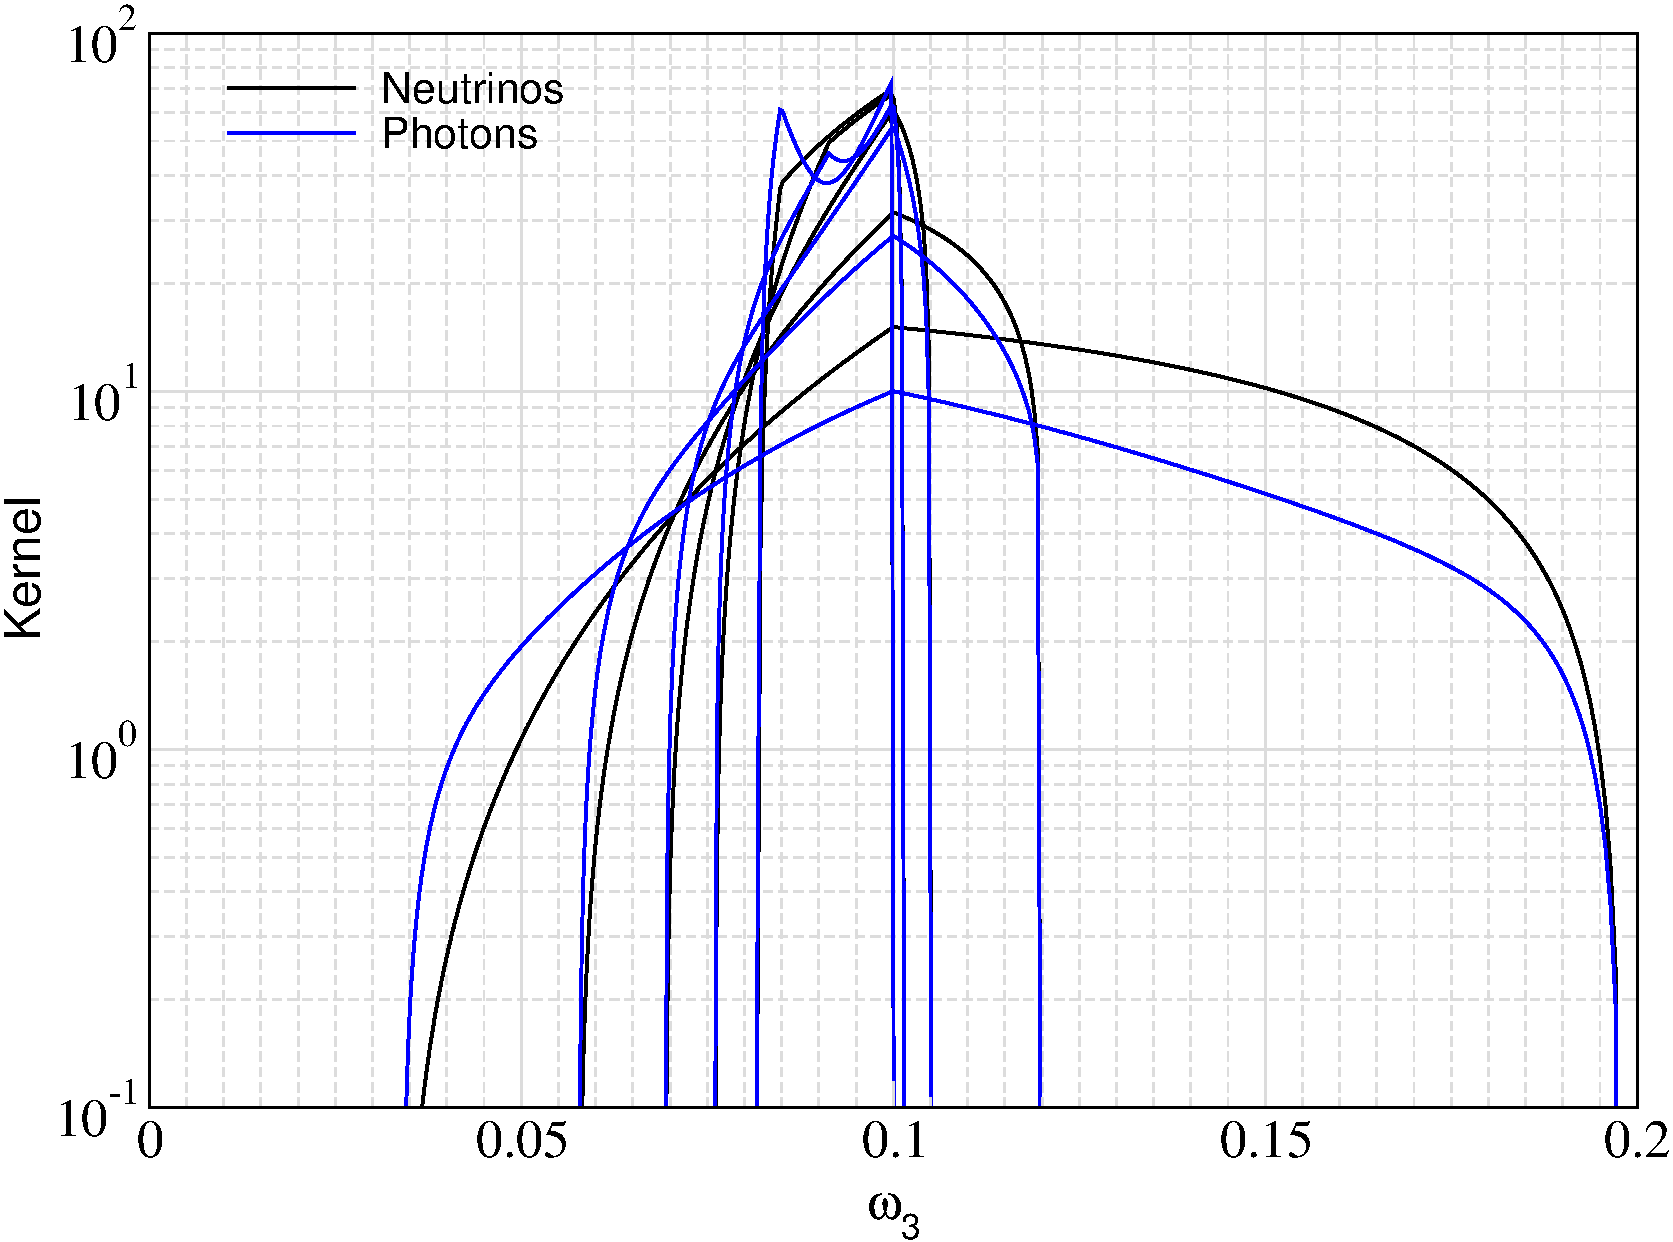
\includegraphics[width=0.88\linewidth]{Kernel_nu_ph.pdf}
\caption{Fixed-momentum photon and electron-neutrino kernels for the same
incoming energy and selected scatterer momenta.}
\end{figure}

\begin{figure}[htbp]
\centering
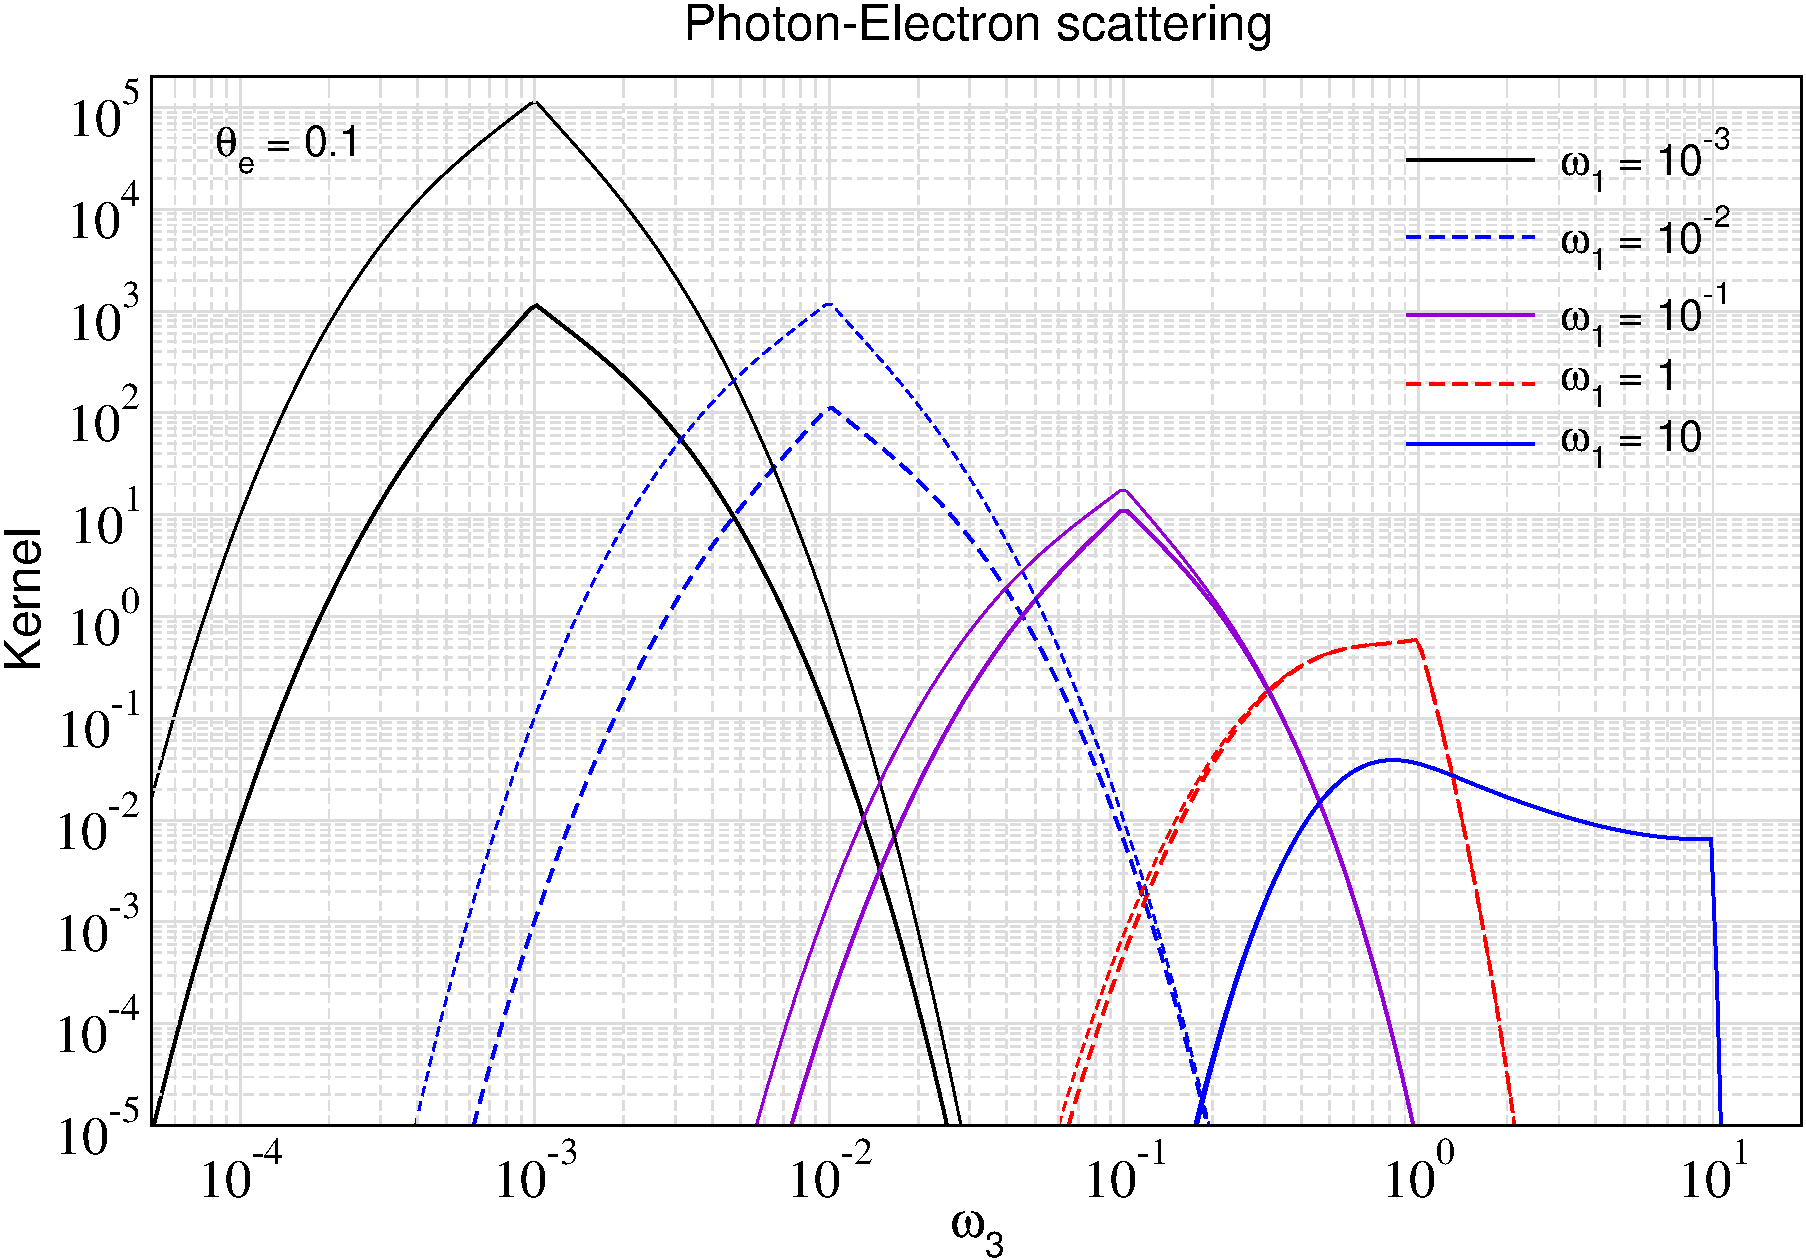
\includegraphics[width=0.88\linewidth]{Kernel_ph_FD.pdf}
\caption{Thermally averaged photon-electron kernels at $\Theta_e=0.1$ for
several incoming energies.}
\end{figure}

\begin{figure}[htbp]
\centering
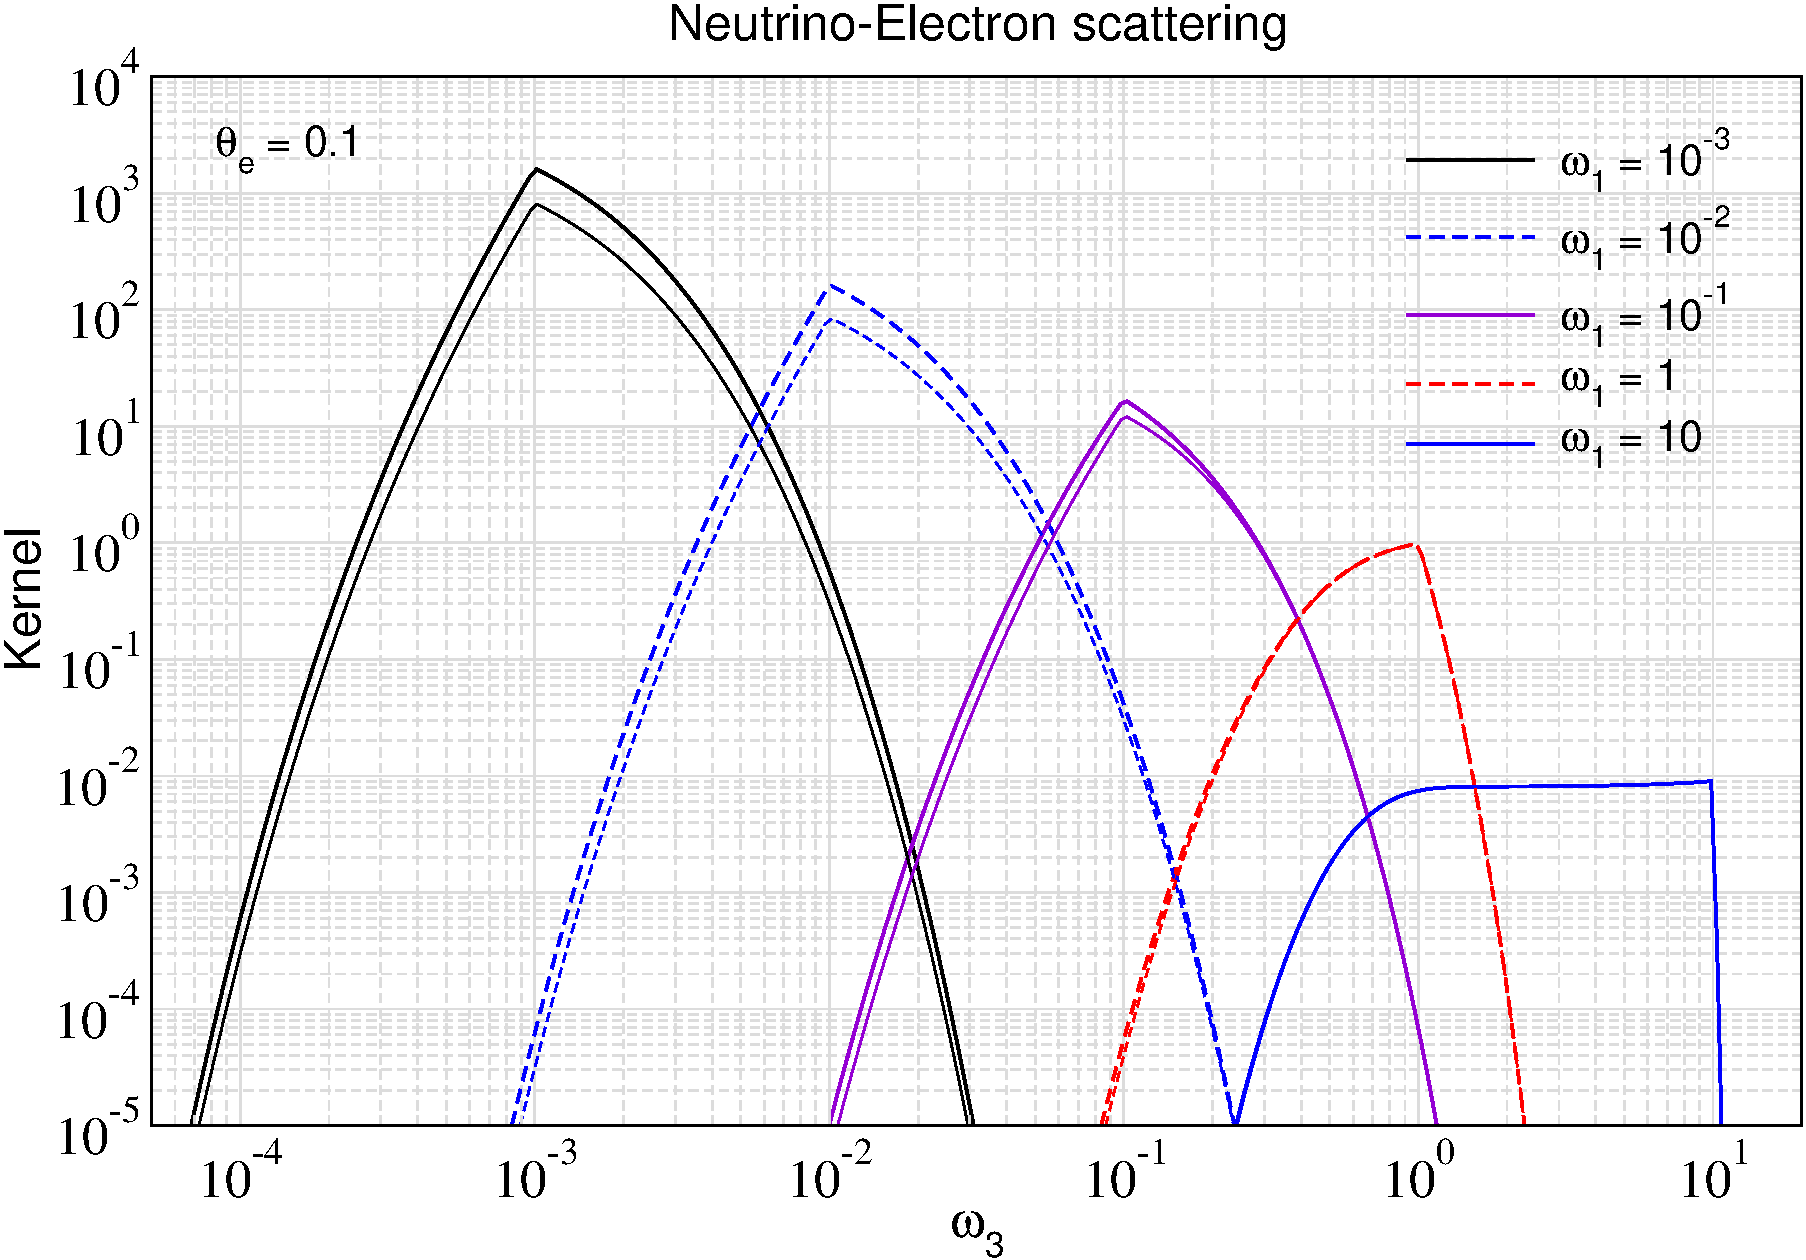
\includegraphics[width=0.88\linewidth]{Kernel_nu_FD.pdf}
\caption{Thermally averaged electron-neutrino kernels at $\Theta_e=0.1$ for the
same incoming-energy sequence.}
\end{figure}

\clearpage
\section{References}

\small
\begin{thebibliography}{9}

\bibitem{SarkarChlubaLee2019}
A.~Sarkar, J.~Chluba and E.~Lee,
``Dissecting the Compton scattering kernel I: Isotropic media,''
Monthly Notices of the Royal Astronomical Society \textbf{490}, 3705--3726
(2019), arXiv:1905.00868.
\url{https://arxiv.org/abs/1905.00868}

\bibitem{ChlubaCyrUwaboNiiboYamaguchi2026}
J.~Chluba, B.~Cyr, M.~Uwabo-Niibo and M.~Yamaguchi,
``Neutrino-electron scattering kernels in isotropic media,''
arXiv:2607.25436.
\url{https://arxiv.org/abs/2607.25436}

\bibitem{SazonovSunyaev2000}
S.~Y. Sazonov and R.~A. Sunyaev,
``Cosmic microwave background radiation in the direction of a moving cluster of
galaxies with hot gas: relativistic corrections,''
Astrophysical Journal \textbf{543}, 28--55 (2000).

\end{thebibliography}

\end{document}
